
\documentclass[english]{cccconf}
%\documentclass[usemulticol,english]{cccconf}
\usepackage[comma,numbers,square,sort&compress]{natbib}
\usepackage{epstopdf}
\begin{document}

\title{Fuel Feed Control for Asymmetric Arranged Multi-tanks Aircraft: A Hybrid MPC Approach}

\author{Haoyu Miao\aref{sustech},
        Mengfan Cao\aref{sustech},
        Shibo Chen\aref{sustech},
        Zaiyue Yang\aref{sustech}}

\affiliation[sustech]{Southern University of Science and Technology, Shenzhen 518055, P.~R.~China
        \email{haoyumiao97@gmail.com, chensb@sustech.edu.cn, yangzy3@sustech.edu.cn}}

\maketitle

\begin{abstract}
Aircraft fuel system, which provides a continuous source of fuel to the engine, is an important component of the aircraft.
Although the sequential fuel feed strategy for the symmetric arranged multi-tanks aircraft is widely used in today's aircraft, the fuel feed strategy of the asymmetric arranged multi-tanks is still a challenge.
In this article, a two layer offline approach is developed to obtain the fuel feed strategy to minimize the difference between the actual center of gravity (CG) and the desired CG.
The performance of the proposed approach is tested in a case study based on the test data of aircraft pitch movement. 
The result indicates that the proposed approach solves the problem with an offline manner from the optimization perspective.

\end{abstract}

\keywords{asymmetric arranged multi-tanks, fuel feed control, hybrid MPC, warm start}

% Please remove or comment out the following line if the footnote is not necessary
\footnotetext{This work is supported by National Natural Science
Foundation (NNSF) of China under Grant 00000000.}

\section{Introduction}

To be completed.



\subsection{Figures}

%\begin{figure}[!htb]
%  \centering
%  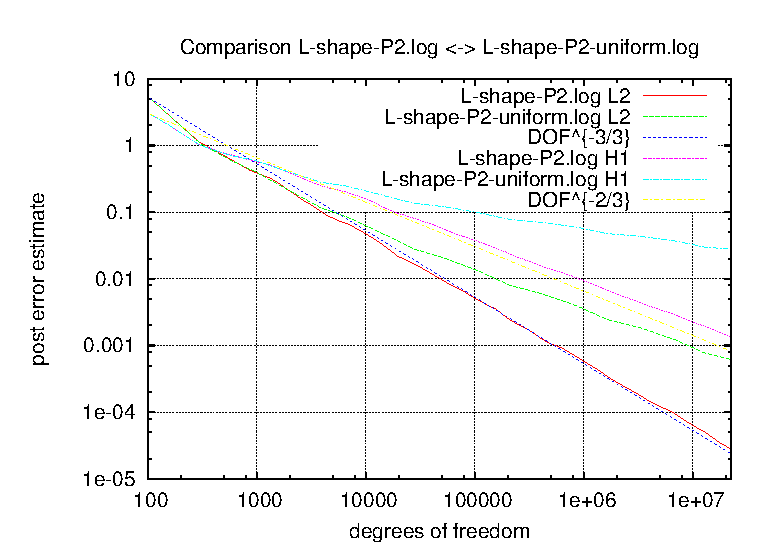
\includegraphics[width=\hsize]{fig1.eps}
%  \caption{The figure caption}
%  \label{fig1}
%\end{figure}

\section{System Model}
The details of the model is refered to \cite{miao2021optimal}.



\section{Problem Formulation}




\section{Methodology}

\section{Experimental Results}

\begin{table}[htbp]
  \caption{Geometric Center Coordinates of Fuel Tanks}
  \begin{center}
  \begin{tabular}{c|c|c|c}
  \hhline
  \textbf{Fuel}&\multicolumn{3}{|c|}{\textbf{Geometric Center Coordinates (Unit:m)}} \\
  \cline{2-4} 
  \textbf{Tank} & \textbf{\textit{x}}& \textbf{\textit{y}}& \textbf{\textit{z}} \\
  \hline
  \#1 & 8.913043& 1.20652174 & 0.61669004\\%$^{\mathrm{a}}$& &  \\
  \#2 & 6.91304348 & -1.39347826 & 0.21669004 \\
  \#3 & -1.68695652 & 1.20652174 & -0.28330996 \\
  \#4 & 3.11304348 & 0.60652174 & -0.18330996\\
  \#5 & -5.28695652 & -0.29347826 & 0.41669004\\
  \#6 & -2.08695652 & -1.49347826 & 0.21669004\\
  \hhline
  %\multicolumn{4}{l}{$^{\mathrm{a}}$Sample of a Table footnote.}
  \end{tabular}
  \label{Table:Geometric Center}
  \end{center}
  \end{table}

\section{Conclusion}


\bibliographystyle{plain}
\bibliography{references}


% \begin{thebibliography}{0}
% \bibitem{cheng2005}
% D.~Cheng, Controllability of switched bilinear systems, \emph{IEEE Trans. on
%   Automatic Control}, 50(4): 511--515, 2005.

% \bibitem{poor1985}
% H.~Poor, \emph{An Introduction to Signal Detection and Estimation}. New York: Springer-Verlag, 1985, chapter 4.

% \bibitem{smith}
% B.~Smith, An approach to graphs of linear forms, accepted.

% \bibitem{cheng2005a}
% D.~Cheng, On logic-based intelligent systems, in \emph{Proceedings of 5th
%   International Conference on Control and Automation}, 2005: 71--75.

% \bibitem{cheng2005b}
% D.~Cheng, R.~Ortega, and E.~Panteley, On port controlled hamiltonian systems,
%   in \emph{Advanced Robust and Adaptive Control --- Theory and Applications},
%   D.~Cheng, Y.~Sun, T.~Shen, and H.~Ohmori, Eds. Beijing: Tsinghua University Press, 2005: 3--16.
% \end{thebibliography}

\end{document}

